\subsubsection{Module MD-06: Quản lý Bán mang về (POS - Takeout)}

Module Quản lý Bán mang về (MD-06) là một phần mở rộng hoặc một chế độ hoạt động chuyên biệt của hệ thống Point of Sale (POS), được thiết kế để phục vụ nhu cầu của khách hàng mua đồ ăn, thức uống để mang đi (Takeout/Takeaway). Module này tập trung vào việc xử lý nhanh chóng các đơn hàng không yêu cầu quản lý bàn, từ việc tạo đơn, chọn món, cho đến thanh toán và hoàn tất giao dịch.

\begin{figure}[H]
    \centering
    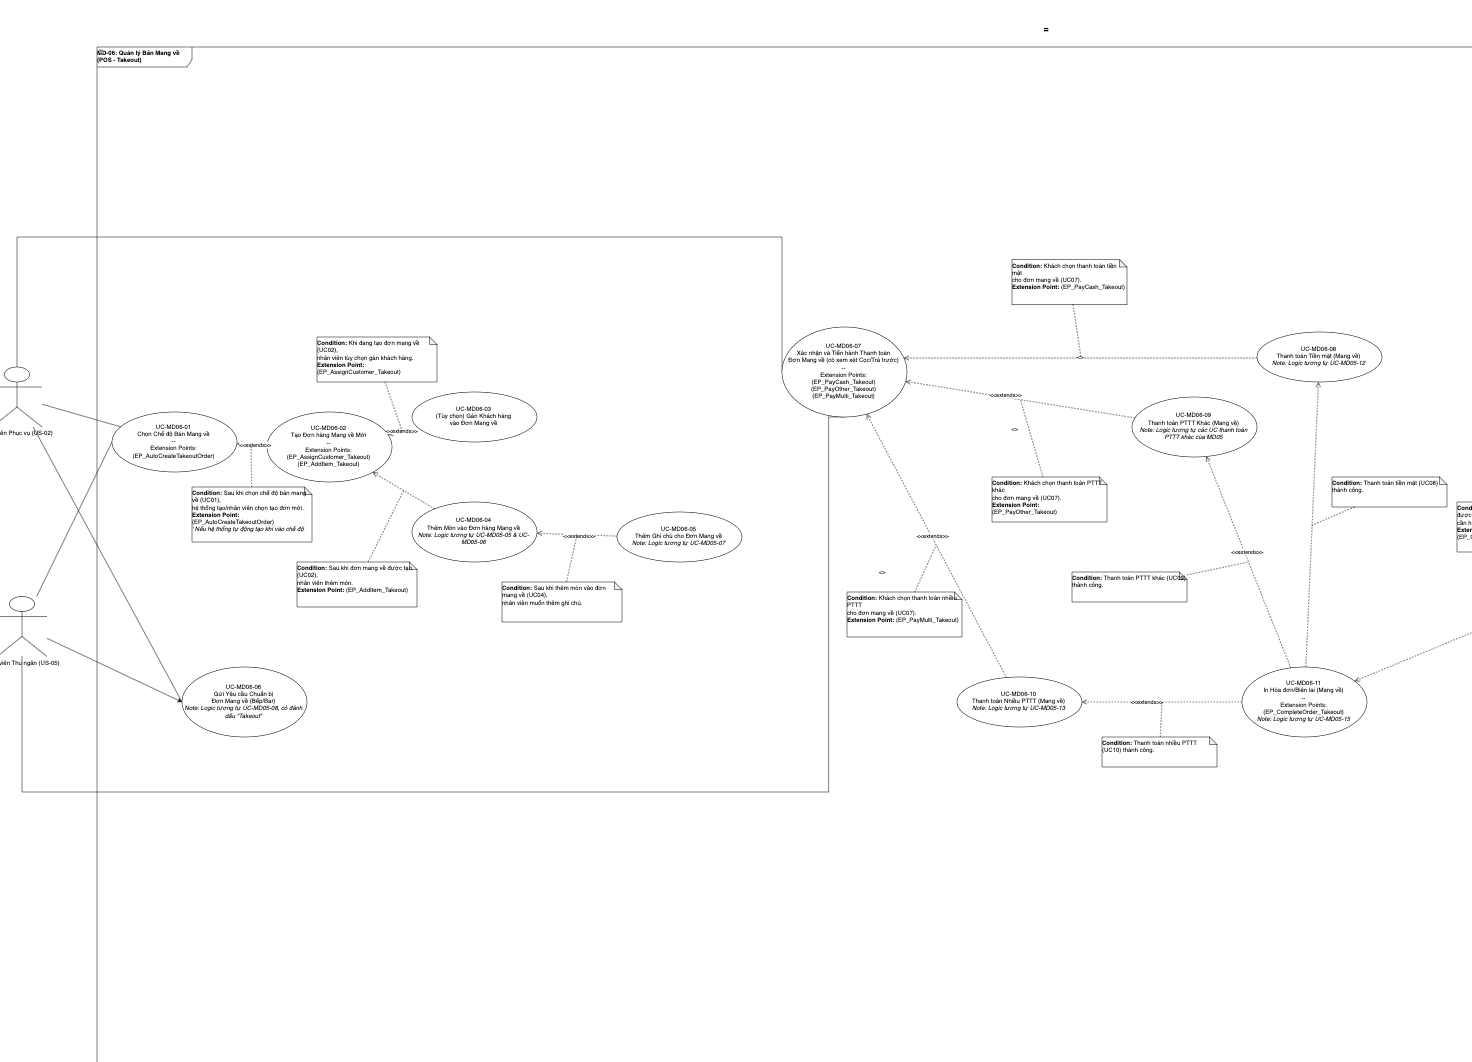
\includegraphics[width=15cm]{Sections/tong_quan/functional_spec/img/uc6.png}
    \vspace{0.5cm}
    \caption{Use case diagram cho Module MD-06}
    \label{fig:my_label}
\end{figure}

\begin{longtable}{|m{2cm}|m{2.5cm}|m{2.5cm}|m{4.5cm}|m{4cm}|}
\caption{Danh sách Yêu cầu Chức năng cho Module MD-06: Quản lý Bán hàng Mang về (POS - Takeout)} \label{tab:fr_md06_revised_v3} \\
\hline
\textbf{Mã Module} & \textbf{Mã Yêu cầu CN} & \textbf{Mã Người dùng} & \textbf{Tên Chức năng} & \textbf{Mô tả Ngắn} \\
\hline
\endhead % Header cho các trang tiếp theo
\hline
\endfoot % Footer cho bảng
\hline
\endlastfoot % Footer cho trang cuối cùng

MD-06 & FR-MD06-01 & US-02, US-05 & Chọn Chế độ Bán Mang về & Nhân viên chọn chế độ/giao diện riêng trên POS cho đơn mang về. \\
\hline
MD-06 & FR-MD06-02 & US-02, US-05 & Tạo Đơn hàng Mang về Mới & Nhân viên khởi tạo một đơn hàng mới trong chế độ mang về. \\
\hline
MD-06 & FR-MD06-03 & US-02, US-05 & Gán Khách hàng vào Đơn Mang về & Nhân viên tìm và liên kết đơn mang về với khách hàng có sẵn hoặc tạo mới. \\
\hline
MD-06 & FR-MD06-04 & US-02, US-05 & Thêm Món vào Đơn hàng Mang về & Nhân viên thêm món ăn/đồ uống vào đơn hàng mang về. (Hành động tương tự FR-MD05-05, FR-MD05-06). \\
\hline
MD-06 & FR-MD06-05 & US-02, US-05 & Thêm Ghi chú cho Đơn Mang về & Nhân viên thêm ghi chú đặc biệt cho món hoặc cả đơn mang về. (Hành động tương tự FR-MD05-07). \\
\hline
MD-06 & FR-MD06-06 & US-02, US-05 & Gửi Yêu cầu Chuẩn bị Đơn Mang về (Bếp/Bar) & Nhân viên gửi thông tin món cần chuẩn bị đến bếp/bar, có đánh dấu "Takeout". (Hành động tương tự FR-MD05-08). \\
\hline
MD-06 & FR-MD06-07 & US-02, US-05 & Xác nhận và Tiến hành Thanh toán Đơn Mang về (có xem xét Cọc/Trả trước) & Nhân viên vào màn hình thanh toán, nơi hệ thống đã tự động áp dụng cọc/trả trước (nếu đơn hàng được đặt online và có trả trước). \\
\hline
MD-06 & FR-MD06-08 & US-02, US-05 & Thực hiện Thanh toán Tiền mặt cho Đơn Mang về & Nhân viên nhận tiền mặt và ghi nhận thanh toán. (Hành động tương tự FR-MD05-12). \\
\hline
MD-06 & FR-MD06-09 & US-02, US-05 & Ghi nhận Thanh toán bằng Phương thức Khác (Không Thẻ) cho Đơn Mang về & Nhân viên ghi nhận thanh toán bằng các phương thức khác được hỗ trợ (ví dụ: ví điện tử nếu có). \\
\hline
MD-06 & FR-MD06-10 & US-02, US-05 & Thực hiện Thanh toán Đơn Mang về bằng Nhiều Phương thức (Không Thẻ) & Nhân viên nhận thanh toán bằng cách kết hợp nhiều phương thức được hỗ trợ. (Hành động tương tự FR-MD05-13). \\
\hline
MD-06 & FR-MD06-11 & US-02, US-05 & In Hóa đơn/Biên lai cho Đơn Mang về & Nhân viên kích hoạt in hóa đơn/biên lai sau khi thanh toán. (Hành động tương tự FR-MD05-15). \\
\hline
MD-06 & FR-MD06-12 & US-02, US-05 & Hoàn tất Đơn hàng Mang về & Nhân viên đóng đơn hàng mang về sau khi khách đã thanh toán và nhận hàng. (Hành động tương tự FR-MD05-16). \\
\hline

\end{longtable}


\subsubsubsection{Mục tiêu và Phạm vi}
\label{sssec:md06_objectives_scope}
Mục tiêu chính của module MD-06 là:
\begin{itemize}
    \item \textbf{Xử lý nhanh đơn hàng mang về:} Cung cấp một quy trình tinh gọn cho nhân viên để tiếp nhận và xử lý các đơn hàng mang đi một cách hiệu quả, giảm thời gian chờ đợi cho khách hàng.
    \item \textbf{Quản lý đơn hàng không cần bàn:} Cho phép tạo và quản lý các đơn hàng mà không cần liên kết với một bàn cụ thể trong nhà hàng.
    \item \textbf{Tích hợp với quy trình chuẩn bị:} Đảm bảo thông tin đơn hàng mang về được gửi chính xác xuống bếp/bar, có phân biệt rõ ràng với đơn ăn tại bàn để bộ phận chuẩn bị có quy trình đóng gói phù hợp.
    \item \textbf{Linh hoạt trong việc gán khách hàng (tùy chọn):} Cho phép liên kết đơn hàng với thông tin khách hàng để tiện theo dõi hoặc áp dụng các chương trình khuyến mãi.
    \item \textbf{Hỗ trợ thanh toán đa dạng:} Cho phép khách hàng thanh toán bằng nhiều phương thức khác nhau.
    \item \textbf{Xử lý các khoản trả trước/đặt cọc:} Tự động áp dụng các khoản tiền khách hàng có thể đã thanh toán trước khi đặt hàng mang về qua các kênh khác (ví dụ: website, ứng dụng).
\end{itemize}
Phạm vi của module bao gồm từ việc nhân viên chọn chế độ bán mang về, tạo đơn hàng, thêm món, gửi yêu cầu chuẩn bị, cho đến khi xử lý thanh toán và hoàn tất đơn hàng. Module này không bao gồm các chức năng quản lý bàn hoặc đặt chỗ phức tạp như ở module ăn tại bàn (MD-05) hay đặt chỗ (MD-03).

\subsubsubsection{Đối tượng Sử dụng Chính}
\label{sssec:md06_primary_users}
Các đối tượng người dùng chính tương tác với module này bao gồm:
\begin{itemize}
    \item \textbf{US-02 (Nhân viên phục vụ):} Có thể trực tiếp nhận đơn hàng mang về từ khách tại quầy.
    \item \textbf{US-05 (Nhân viên thu ngân):} Thường là người chính xử lý các đơn hàng mang về, bao gồm việc tạo đơn, nhận thanh toán và hoàn tất giao dịch.
    \item \textbf{US-01 (Quản lý nhà hàng):} Có thể sử dụng các chức năng này và giám sát hoạt động bán mang về.
\end{itemize}
Khách hàng (US-08) là người yêu cầu dịch vụ mang về và cung cấp thông tin đơn hàng.

\subsubsubsection{Các Chức năng Chính}
\label{sssec:md06_key_functionalities}
Module MD-06 cung cấp các chức năng cần thiết để quản lý hiệu quả quy trình bán mang về, được mô tả chi tiết qua các Use Case sau:

\begin{itemize}
    \item \textbf{Khởi tạo và Quản lý Đơn hàng Mang về (UC-MD06-01 đến UC-MD06-03):}
    \begin{itemize}
        \item Cho phép nhân viên chủ động chọn hoặc chuyển sang chế độ hoạt động dành riêng cho bán mang về trên giao diện POS (UC-MD06-01).
        \item Hệ thống tự động hoặc nhân viên khởi tạo một đơn hàng POS mới, được đánh dấu là loại hình "Mang về" (UC-MD06-02).
        \item (Tùy chọn) Cho phép nhân viên tìm kiếm khách hàng đã có hoặc tạo nhanh thông tin khách hàng mới để liên kết với đơn hàng mang về (UC-MD06-03).
    \end{itemize}

    \item \textbf{Thao tác trên Đơn hàng Mang về (UC-MD06-04 đến UC-MD06-06):}
    \begin{itemize}
        \item Thêm các món ăn/đồ uống vào đơn hàng mang về, bao gồm việc chọn biến thể và điều chỉnh số lượng (UC-MD06-04, tương tự UC-MD05-05 và UC-MD05-06).
        \item Thêm các ghi chú hoặc yêu cầu đặc biệt của khách (ví dụ: về đóng gói, khẩu vị) cho từng món hoặc toàn bộ đơn hàng mang về (UC-MD06-05, tương tự UC-MD05-07).
        \item Gửi thông tin các món đã chọn của đơn hàng mang về xuống các máy in bếp/bar hoặc màn hình KDS, có chỉ dẫn rõ đây là đơn mang về (UC-MD06-06, tương tự UC-MD05-08 nhưng có thêm thông tin "Takeout").
    \end{itemize}

    \item \textbf{Xử lý Thanh toán cho Đơn hàng Mang về (UC-MD06-07 đến UC-MD06-12):}
    \begin{itemize}
        \item Trước khi vào màn hình thanh toán, hệ thống tự động kiểm tra và áp dụng (trừ đi) các khoản tiền đặt cọc hoặc thanh toán trước mà khách hàng có thể đã thực hiện cho đơn hàng mang về đó (UC-MD06-07).
        \item Thực hiện thanh toán bằng tiền mặt cho đơn hàng mang về (UC-MD06-08, tương tự UC-MD05-12).
        \item Ghi nhận thanh toán bằng các phương thức khác được hỗ trợ (không bao gồm thẻ ngân hàng qua terminal tích hợp) cho đơn hàng mang về (UC-MD06-09, tương tự UC-MD05-13).
        \item Thực hiện thanh toán cho đơn hàng mang về bằng cách kết hợp nhiều phương thức khác nhau (không bao gồm thẻ) (UC-MD06-10, tương tự UC-MD05-14).
        \item Sau khi nhận đủ thanh toán, cho phép nhân viên kích hoạt (hoặc hệ thống tự động) in hóa đơn/biên lai cuối cùng cho đơn hàng mang về (UC-MD06-11, tương tự UC-MD05-16).
        \item Hoàn tất và đóng đơn hàng mang về trong hệ thống sau khi khách đã thanh toán và nhận hàng (UC-MD06-12, tương tự UC-MD05-17).
    \end{itemize}
\end{itemize}

\subsubsubsection{Tóm tắt Luồng Hoạt động Tổng thể}
\label{sssec:md06_overall_workflow}
Luồng hoạt động điển hình trong module Bán mang về (POS - Takeout) diễn ra như sau:
\begin{enumerate}
    \item \textbf{Chuyển sang chế độ mang về:} Nhân viên Chọn Chế độ Bán Mang về (UC-MD06-01) trên giao diện POS.
    \item \textbf{Tạo đơn hàng:} Hệ thống tự động hoặc nhân viên Tạo Đơn hàng Mang về Mới (UC-MD06-02).
    \item \textbf{(Tùy chọn) Gán khách hàng:} Nhân viên Gán Khách hàng vào Đơn Mang về (UC-MD06-03).
    \item \textbf{Nhập món ăn:}
        \begin{itemize}
            \item Nhân viên Thêm Món vào Đơn hàng Mang về (UC-MD06-04).
            \item Thêm Ghi chú cho Đơn Mang về (UC-MD06-05) nếu khách có yêu cầu đặc biệt.
        \end{itemize}
    \item \textbf{Gửi yêu cầu chuẩn bị:} Nhân viên Gửi Yêu cầu Chuẩn bị Đơn Mang về (Bếp/Bar) (UC-MD06-06), phiếu gửi đi có ghi rõ là "Takeout".
    \item \textbf{Tiến hành thanh toán:}
        \begin{itemize}
            \item Nhân viên chọn thanh toán, hệ thống Xác nhận và Tiến hành Thanh toán Đơn Mang về, có xem xét và tự động áp dụng Cọc/Trả trước nếu có (UC-MD06-07).
            \item Nhân viên nhận thanh toán bằng một hoặc nhiều phương thức: Tiền mặt (UC-MD06-08), Phương thức Khác (Không Thẻ) (UC-MD06-09), hoặc kết hợp Nhiều Phương thức (Không Thẻ) (UC-MD06-10).
        \end{itemize}
    \item \textbf{Hoàn tất giao dịch:}
        \begin{itemize}
            \item Sau khi thanh toán đủ, nhân viên In Hóa đơn/Biên lai cho Đơn Mang về (UC-MD06-11).
            \item Cuối cùng, nhân viên Hoàn tất Đơn hàng Mang về (UC-MD06-12) trong hệ thống.
        \end{itemize}
\end{enumerate}
Module MD-06 đảm bảo rằng các đơn hàng mang về được xử lý một cách nhanh chóng, chính xác và hiệu quả, đáp ứng nhu cầu của cả khách hàng và nhà hàng.

